% Options for packages loaded elsewhere
\PassOptionsToPackage{unicode}{hyperref}
\PassOptionsToPackage{hyphens}{url}
\PassOptionsToPackage{dvipsnames,svgnames,x11names}{xcolor}
%
\documentclass[
  letterpaper,
]{krantz}

\usepackage{amsmath,amssymb}
\usepackage{iftex}
\ifPDFTeX
  \usepackage[T1]{fontenc}
  \usepackage[utf8]{inputenc}
  \usepackage{textcomp} % provide euro and other symbols
\else % if luatex or xetex
  \usepackage{unicode-math}
  \defaultfontfeatures{Scale=MatchLowercase}
  \defaultfontfeatures[\rmfamily]{Ligatures=TeX,Scale=1}
\fi
\usepackage{lmodern}
\ifPDFTeX\else  
    % xetex/luatex font selection
\fi
% Use upquote if available, for straight quotes in verbatim environments
\IfFileExists{upquote.sty}{\usepackage{upquote}}{}
\IfFileExists{microtype.sty}{% use microtype if available
  \usepackage[]{microtype}
  \UseMicrotypeSet[protrusion]{basicmath} % disable protrusion for tt fonts
}{}
\makeatletter
\@ifundefined{KOMAClassName}{% if non-KOMA class
  \IfFileExists{parskip.sty}{%
    \usepackage{parskip}
  }{% else
    \setlength{\parindent}{0pt}
    \setlength{\parskip}{6pt plus 2pt minus 1pt}}
}{% if KOMA class
  \KOMAoptions{parskip=half}}
\makeatother
\usepackage{xcolor}
\setlength{\emergencystretch}{3em} % prevent overfull lines
\setcounter{secnumdepth}{5}
% Make \paragraph and \subparagraph free-standing
\ifx\paragraph\undefined\else
  \let\oldparagraph\paragraph
  \renewcommand{\paragraph}[1]{\oldparagraph{#1}\mbox{}}
\fi
\ifx\subparagraph\undefined\else
  \let\oldsubparagraph\subparagraph
  \renewcommand{\subparagraph}[1]{\oldsubparagraph{#1}\mbox{}}
\fi


\providecommand{\tightlist}{%
  \setlength{\itemsep}{0pt}\setlength{\parskip}{0pt}}\usepackage{longtable,booktabs,array}
\usepackage{calc} % for calculating minipage widths
% Correct order of tables after \paragraph or \subparagraph
\usepackage{etoolbox}
\makeatletter
\patchcmd\longtable{\par}{\if@noskipsec\mbox{}\fi\par}{}{}
\makeatother
% Allow footnotes in longtable head/foot
\IfFileExists{footnotehyper.sty}{\usepackage{footnotehyper}}{\usepackage{footnote}}
\makesavenoteenv{longtable}
\usepackage{graphicx}
\makeatletter
\def\maxwidth{\ifdim\Gin@nat@width>\linewidth\linewidth\else\Gin@nat@width\fi}
\def\maxheight{\ifdim\Gin@nat@height>\textheight\textheight\else\Gin@nat@height\fi}
\makeatother
% Scale images if necessary, so that they will not overflow the page
% margins by default, and it is still possible to overwrite the defaults
% using explicit options in \includegraphics[width, height, ...]{}
\setkeys{Gin}{width=\maxwidth,height=\maxheight,keepaspectratio}
% Set default figure placement to htbp
\makeatletter
\def\fps@figure{htbp}
\makeatother
% definitions for citeproc citations
\NewDocumentCommand\citeproctext{}{}
\NewDocumentCommand\citeproc{mm}{%
  \begingroup\def\citeproctext{#2}\cite{#1}\endgroup}
\makeatletter
 % allow citations to break across lines
 \let\@cite@ofmt\@firstofone
 % avoid brackets around text for \cite:
 \def\@biblabel#1{}
 \def\@cite#1#2{{#1\if@tempswa , #2\fi}}
\makeatother
\newlength{\cslhangindent}
\setlength{\cslhangindent}{1.5em}
\newlength{\csllabelwidth}
\setlength{\csllabelwidth}{3em}
\newenvironment{CSLReferences}[2] % #1 hanging-indent, #2 entry-spacing
 {\begin{list}{}{%
  \setlength{\itemindent}{0pt}
  \setlength{\leftmargin}{0pt}
  \setlength{\parsep}{0pt}
  % turn on hanging indent if param 1 is 1
  \ifodd #1
   \setlength{\leftmargin}{\cslhangindent}
   \setlength{\itemindent}{-1\cslhangindent}
  \fi
  % set entry spacing
  \setlength{\itemsep}{#2\baselineskip}}}
 {\end{list}}
\usepackage{calc}
\newcommand{\CSLBlock}[1]{\hfill\break\parbox[t]{\linewidth}{\strut\ignorespaces#1\strut}}
\newcommand{\CSLLeftMargin}[1]{\parbox[t]{\csllabelwidth}{\strut#1\strut}}
\newcommand{\CSLRightInline}[1]{\parbox[t]{\linewidth - \csllabelwidth}{\strut#1\strut}}
\newcommand{\CSLIndent}[1]{\hspace{\cslhangindent}#1}

\usepackage{booktabs}
\usepackage{longtable}
\usepackage[bf,singlelinecheck=off]{caption}
\usepackage[scale=.8]{sourcecodepro}
\usepackage{hyperref}

\usepackage{framed,color}
\definecolor{shadecolor}{RGB}{248,248,248}

\renewcommand{\textfraction}{0.05}
\renewcommand{\topfraction}{0.8}
\renewcommand{\bottomfraction}{0.8}
\renewcommand{\floatpagefraction}{0.75}

\renewenvironment{quote}{\begin{VF}}{\end{VF}}
\let\oldhref\href
\renewcommand{\href}[2]{#2\footnote{\url{#1}}}

\makeatletter
\newenvironment{kframe}{%
\medskip{}
\setlength{\fboxsep}{.8em}
 \def\at@end@of@kframe{}%
 \ifinner\ifhmode%
  \def\at@end@of@kframe{\end{minipage}}%
  \begin{minipage}{\columnwidth}%
 \fi\fi%
 \def\FrameCommand##1{\hskip\@totalleftmargin \hskip-\fboxsep
 \colorbox{shadecolor}{##1}\hskip-\fboxsep
     % There is no \\@totalrightmargin, so:
     \hskip-\linewidth \hskip-\@totalleftmargin \hskip\columnwidth}%
 \MakeFramed {\advance\hsize-\width
   \@totalleftmargin\z@ \linewidth\hsize
   \@setminipage}}%
 {\par\unskip\endMakeFramed%
 \at@end@of@kframe}
\makeatother



%\renewenvironment{Shaded}{\begin{kframe}}{\end{kframe}}

\usepackage{makeidx}
\makeindex

\urlstyle{tt}

\usepackage{amsthm}
\makeatletter
\def\thm@space@setup{%
  \thm@preskip=8pt plus 2pt minus 4pt
  \thm@postskip=\thm@preskip
}
\makeatother

\frontmatter
\makeatletter
\@ifpackageloaded{bookmark}{}{\usepackage{bookmark}}
\makeatother
\makeatletter
\@ifpackageloaded{caption}{}{\usepackage{caption}}
\AtBeginDocument{%
\ifdefined\contentsname
  \renewcommand*\contentsname{Table of contents}
\else
  \newcommand\contentsname{Table of contents}
\fi
\ifdefined\listfigurename
  \renewcommand*\listfigurename{List of Figures}
\else
  \newcommand\listfigurename{List of Figures}
\fi
\ifdefined\listtablename
  \renewcommand*\listtablename{List of Tables}
\else
  \newcommand\listtablename{List of Tables}
\fi
\ifdefined\figurename
  \renewcommand*\figurename{Figure}
\else
  \newcommand\figurename{Figure}
\fi
\ifdefined\tablename
  \renewcommand*\tablename{Table}
\else
  \newcommand\tablename{Table}
\fi
}
\@ifpackageloaded{float}{}{\usepackage{float}}
\floatstyle{ruled}
\@ifundefined{c@chapter}{\newfloat{codelisting}{h}{lop}}{\newfloat{codelisting}{h}{lop}[chapter]}
\floatname{codelisting}{Listing}
\newcommand*\listoflistings{\listof{codelisting}{List of Listings}}
\makeatother
\makeatletter
\makeatother
\makeatletter
\@ifpackageloaded{caption}{}{\usepackage{caption}}
\@ifpackageloaded{subcaption}{}{\usepackage{subcaption}}
\makeatother
\ifLuaTeX
  \usepackage{selnolig}  % disable illegal ligatures
\fi
\usepackage{bookmark}

\IfFileExists{xurl.sty}{\usepackage{xurl}}{} % add URL line breaks if available
\urlstyle{same} % disable monospaced font for URLs
\hypersetup{
  pdftitle={Our name},
  pdfauthor={Zobitz and Zimmerman},
  colorlinks=true,
  linkcolor={blue},
  filecolor={Maroon},
  citecolor={Blue},
  urlcolor={Blue},
  pdfcreator={LaTeX via pandoc}}

\title{Our name}
\author{Zobitz and Zimmerman}
\date{2024-12-02}

\begin{document}
\maketitle

% you may need to leave a few empty pages before the dedication page

%\cleardoublepage\newpage\thispagestyle{empty}\null
%\cleardoublepage\newpage\thispagestyle{empty}\null
%\cleardoublepage\newpage
\thispagestyle{empty}

\begin{center}
%\includegraphics{images/dedication.pdf}
\end{center}

\setlength{\abovedisplayskip}{-5pt}
\setlength{\abovedisplayshortskip}{-5pt}

\renewcommand*\contentsname{Table of contents}
{
\hypersetup{linkcolor=}
\setcounter{tocdepth}{2}
\tableofcontents
}
\bookmarksetup{startatroot}

\chapter*{Welcome}\label{welcome}
\addcontentsline{toc}{chapter}{Welcome}

\markboth{Welcome}{Welcome}

Welcome

\mainmatter

\bookmarksetup{startatroot}

\chapter{Environments for Data Science}\label{sec-03environments}

You have data from an experiment, or perhaps have accessed data from an
ecological network such as NEON. You are now ready to explore your data
through visualization, conduct statistical tests, and perhaps increase
the explanatory power beyond just the data collection itself. Your next
step is to choose a computational environment for analysis. As described
in the \textbf{?@sec-02data}, half the battle is loading in data into
your computer and connecting up these datasets. A typical next step is
exploratory data analysis.

This chapter provides contrasts three of the most common programming
languages for data science when faced with a common task. Borrowing
language from ecology, an environment for data science as an
interconnected system with a particular programming language as the
foundation. Just like natural environments, environments for data
science differ depending on the programming language. Let's begin.

\section{Choosing different
languages}\label{choosing-different-languages}

We define an environment for data science as a programming language.
Examples of programming languages include R\index{R},
python\index{python}, julia\index{julia} briefly described in
Table~\ref{tbl-dst-languages}

\begin{longtable}[]{@{}
  >{\raggedright\arraybackslash}p{(\columnwidth - 6\tabcolsep) * \real{0.1538}}
  >{\raggedright\arraybackslash}p{(\columnwidth - 6\tabcolsep) * \real{0.1538}}
  >{\raggedright\arraybackslash}p{(\columnwidth - 6\tabcolsep) * \real{0.4615}}
  >{\raggedright\arraybackslash}p{(\columnwidth - 6\tabcolsep) * \real{0.2308}}@{}}
\caption{Comparison of different programming languages used in data
science.}\label{tbl-dst-languages}\tabularnewline
\toprule\noalign{}
\begin{minipage}[b]{\linewidth}\raggedright
Name
\end{minipage} & \begin{minipage}[b]{\linewidth}\raggedright
First Available
\end{minipage} & \begin{minipage}[b]{\linewidth}\raggedright
Description
\end{minipage} & \begin{minipage}[b]{\linewidth}\raggedright
Reference
\end{minipage} \\
\midrule\noalign{}
\endfirsthead
\toprule\noalign{}
\begin{minipage}[b]{\linewidth}\raggedright
Name
\end{minipage} & \begin{minipage}[b]{\linewidth}\raggedright
First Available
\end{minipage} & \begin{minipage}[b]{\linewidth}\raggedright
Description
\end{minipage} & \begin{minipage}[b]{\linewidth}\raggedright
Reference
\end{minipage} \\
\midrule\noalign{}
\endhead
\bottomrule\noalign{}
\endlastfoot
R & 1993 & Started as a statistical programming language. Contributed
packages allow for the extension of the base language into other data
science programs. & \url{https://www.r-project.org/} \\
python & 1991 & Started as a computer programming language that supports
object-oriented programming. Similar to R, contributed modules extend
the core python language to machine learning, data visualization, and
other areas of science, engineering, and mathematics. &
\url{https://www.python.org/} \\
julia & 2012 & with the goal of combining speed and parallel language
operation, essentially taking the best aspects of different programming
languages and combining into one (al n.d.). &
\url{https://julialang.org/} \\
\end{longtable}

As data scientists we are fortunate the variety of these programming
languages exist! While one programming language may be preferable in
some contexts than others, we should pick the tool that is suited to
gain the best insight from that for what we need in the moment.

This textbook takes a neutral approach on \emph{which} language makes
the most sense (admittedly both of us have our favo\textbf{R}ites).
Rather, let's examine differences between common environmental data
science languages using the power of chatGPT.

Generative AI is an offshoot of machine learning methods from data
science, and so provides a good case study to examine differences
environments for data science. These artificial intelligence tools
(e.g.~\href{https://chat.openai.com/}{chatGPT} and others) have rapidly
transformed our daily lives (especially post 2023) and how we interact
with the internet. For scientific research disclosing the use of
generative AI tools is recognized as maintaining scientific integrity
(Bockting et al. 2023; {``Best {Practices} for {Generative AI} in
{Research} {\textbar} {AJE}''} n.d.; Bertolo and Antonelli 2024). Let's
use them here to contrast how the different environments in
Table~\ref{tbl-dst-languages} produce output.

If we chose R, a prompt to chatGPT might be the following
Figure~\ref{fig-jz-chatgpt}:

\begin{figure}

\centering{

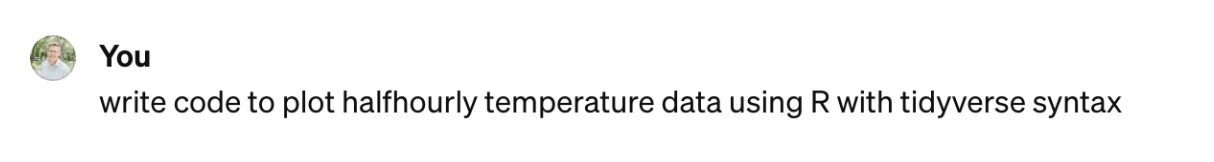
\includegraphics[width=0.9\textwidth,height=\textheight]{images/03_env_data_sci/jz_chatgpt.png}

}

\caption{\label{fig-jz-chatgpt}An innocent question to chatGPT.}

\end{figure}%

Figure~\ref{fig-chatgpt-r} shows its response, which (admittedly) a
well-organized (and documented!) explanation of starter code:

\begin{figure}

\centering{

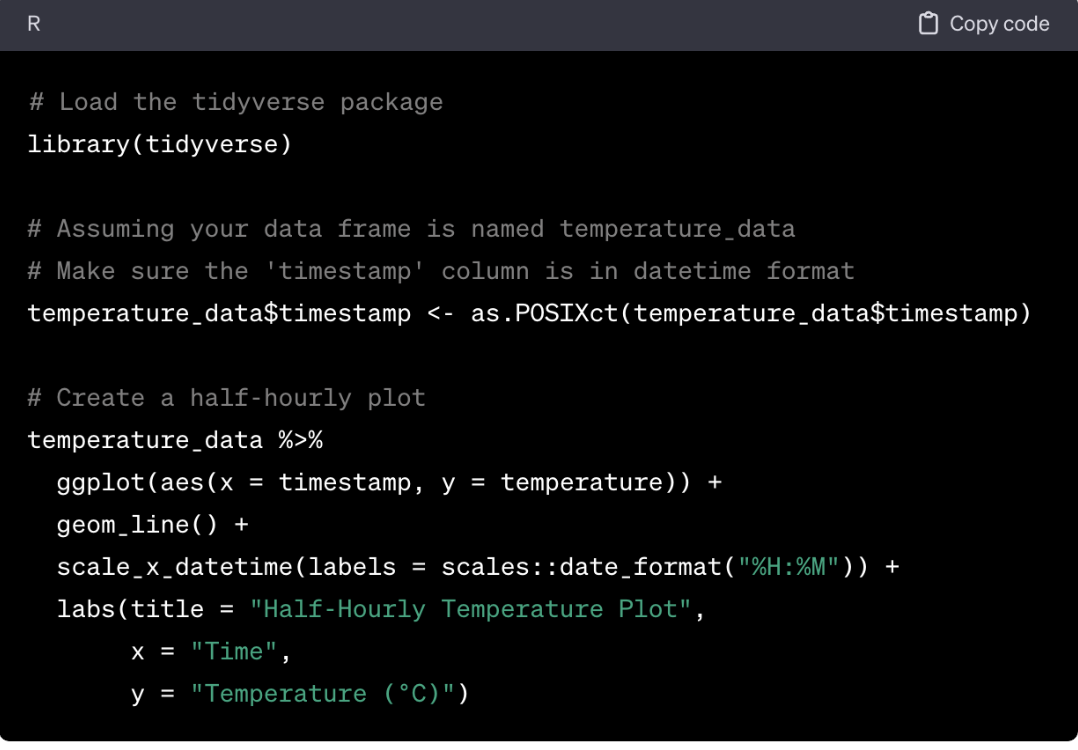
\includegraphics[width=0.9\textwidth,height=\textheight]{images/03_env_data_sci/chatgpt_r.png}

}

\caption{\label{fig-chatgpt-r}How chatGPT responded to our question
using R.}

\end{figure}%

The provided code loads up the correct library (tidyverse), converts the
time to the POSIXct format (which makes working with dates and times
easier) and generates a well-labeled plot. Not too shabby. Based on your
knowledge of R, we would also award extra credit points for using the
tidyverse pipe (\texttt{\%\textgreater{}\%}) in the code, but perhaps
not full credit because of the adoption of the
\href{https://www.tidyverse.org/blog/2023/04/base-vs-magrittr-pipe/}{base
R pipe} (\texttt{\textbar{}\textgreater{}}).

Now let's give the same prompt with python
(Figure~\ref{fig-chatgpt-python}):

\begin{figure}

\centering{

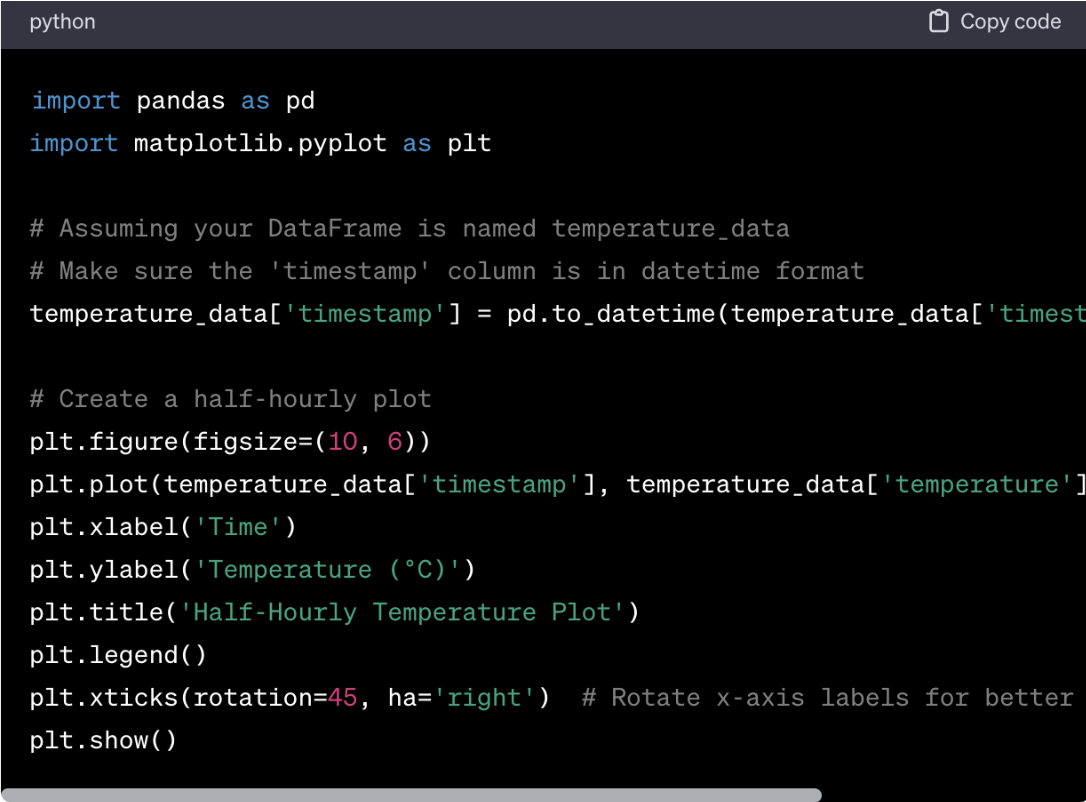
\includegraphics[width=0.9\textwidth,height=\textheight]{images/03_env_data_sci/chatgpt_python.png}

}

\caption{\label{fig-chatgpt-python}How chatGPT responded to our question
with python.}

\end{figure}%

Examining the code seems like a beat for beat rehash of the same code
with R, but with just python (almost like
\href{https://www.vox.com/2015/12/26/10664834/star-force-awakens-derivative}{Star
Wars: The Force Awakens}, but don't @ us!). There are some differences
to note:

\begin{itemize}
\tightlist
\item
  Similar to R, in python libraries are defined at the start of the code
  (with import). However, those libraries need to be referred to when
  you wish to use a command from a particular library (e.g.~the function
  to\_datetime is a function in the pandas library). Thankfully in
  python you can abbreviate the names as pd - whichever makes sense for
  you. (NOTE: In R if you only want to use a particular function in a
  library, then refer to it with the double colon (::,
  e.g.~PACKAGE::FUNCTION) ).
\item
  Python doesn't have the native pipe operator (\textbar\textgreater)
  like R. The assignment operator is equals (=) versus a left facing
  arrow (\textless---).
\end{itemize}

We finally asked chatGPT the same prompt, this time with julia
(Figure~\ref{fig-chatgpt-julia}):

\begin{figure}

\centering{

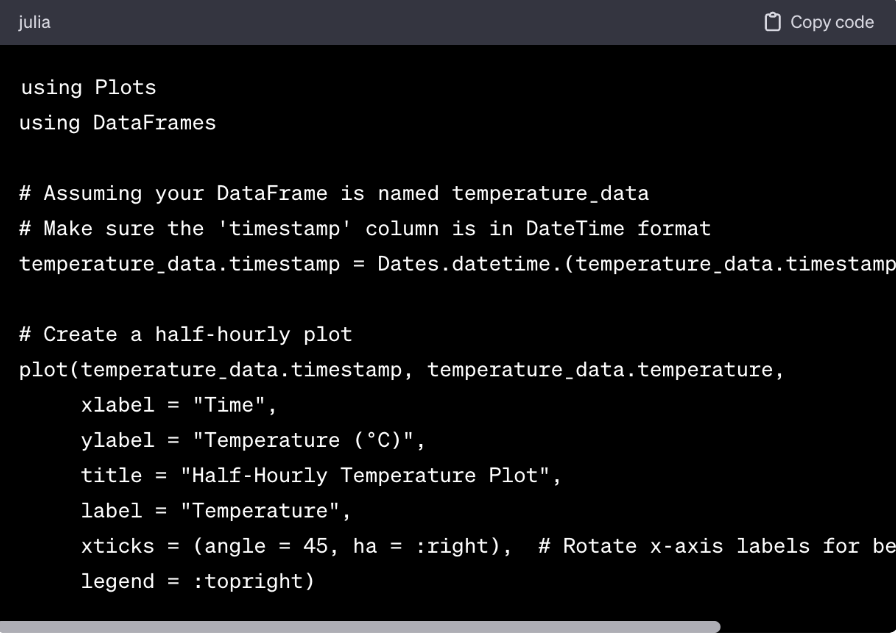
\includegraphics[width=0.9\textwidth,height=\textheight]{images/03_env_data_sci/chatgpt_julia.png}

}

\caption{\label{fig-chatgpt-julia}How chatGPT responded to our question
using julia.}

\end{figure}%

Can you spot the differences (and similarities) with the Julia output in
Figure~\ref{fig-chatgpt-julia} compared to R
(Figure~\ref{fig-chatgpt-r}) or Python
(Figure~\ref{fig-chatgpt-python})? For all practical purposes, it comes
down to preference - which one you are more familiar with.

So which should you choose? R is good for statistics and data
manipulation. There is a strong user base in ecology (Lai et al. 2019).
At the same time, the tidyverse and associated packages have been
developed with data science in mind (Wickham and Grolemund 2017; Wickham
et al. 2019).

The same case could be made for python - which at its core is a
programming language (R was initially designed for statistical analysis
which has morphed into wider applications for data science). If you are
familiar with C or C++, python may feel very familiar to you.

julia is a very promising language with a user base growing in biology
(Roesch et al. 2023). We believe there is longevity in this language,
although it has a smaller user community in the environmental sciences.

A non open-source alternative to programming is
\href{https://www.mathworks.com/products/matlab.html}{MATLAB}, which for
the authors was the first foray into programming languages in graduate
school. This software is used in engineering and industrial
applications. Because it is a commercial and proprietary language, it is
not as translatable for open science applications.
\href{https://octave.org/}{Octave} is an open-source alternative as
MATLAB. From John's experience working with Octave, at the time it was a
good substitute for MATLAB, but it was hard to share code with his
collaborators in biology.

\section{Our recommendations}\label{our-recommendations}

We believe that the best position to take is one of openness to learning
new tools and software as your needs will invariably evolve. It is okay
to dabble! John started out using MATLAB, then transitioned to Octave
because it was open-source. He then moved to work with R (at the same
time as the tidyverse was growing in use) as a fresh start to learn new
tools and techniques for managing data.

Naupaka learned \href{https://en.wikipedia.org/wiki/C\%2B\%2B}{C++} in
high school, then didn't program much until grad school, where I learned
\href{https://www.perl.org/}{perl} in a genomics course. When I started
analyzing my own microbial community ecology data for my dissertation, I
needed the statistical tools only available in R so started teaching
myself. Then along the way I taught myself SQL,
\href{https://www.gnu.org/software/bash/}{bash}, python, and a little
bit of
{[}lisp{]}(https://en.wikipedia.org/wiki/Lisp\_(programming\_language).

\section{The future: why choose?}\label{the-future-why-choose}

Our experiences with programming languages reflect the times we
developed as scientists and the growth of different languages. While we
can't predict the future, but we can safely say at some point you may
use programming language not even mentioned here. Our graduate school
advisors programmed in
\href{https://en.wikipedia.org/wiki/C_(programming_language)}{C} or
\href{https://fortran-lang.org/}{Fortran} - which while still in use,
would not what we would recommend to our students as a first programming
language. Organisms in a biological environment adapt and evolve to
change - and so will you.

Siloing yourself in an particular programming language is becoming less
relevant with the proliferation of online tools such as
\href{https://quarto.org/}{quarto}, \href{https://jupyter.org/}{jupyter
notebooks}, and \href{https://colab.research.google.com/}{google colab}.
These alternatives borrow strengths from each language. We recognize
that code switching can be challenge ({``Comparison of Programming
Languages (Syntax)''} 2024). The best environments for data science
shares a common theme: they are built to support your success and
longevity.

\section{Exercises}\label{exercises}

\begin{enumerate}
\def\labelenumi{\arabic{enumi}.}
\item
  Make an inventory of programming languages you have learned.
\item
  Interview your advisor about what programming languages they used, and
  what they would recommend.
\item
  Give a simple table and give a prompt to import in as a csv and plot
  with a programming language. Compare output. Is it what you would
  expect?
\end{enumerate}

\bookmarksetup{startatroot}

\chapter*{References}\label{references}
\addcontentsline{toc}{chapter}{References}

\markboth{References}{References}

\phantomsection\label{refs}
\begin{CSLReferences}{1}{0}
\bibitem[\citeproctext]{ref-alWhyWeCreated}
al, Viral Shah, Stefan Karpinski. n.d. {``Why {We Created Julia}.''}
https://julialang.org/blog/2012/02/why-we-created-julia/. Accessed April
19, 2024.

\bibitem[\citeproctext]{ref-bertoloGenerativeAIScientific2024}
Bertolo, Riccardo, and Alessandro Antonelli. 2024. {``Generative {AI} in
Scientific Publishing: Disruptive or Destructive?''} \emph{Nature
Reviews Urology} 21 (1): 1--2.
\url{https://doi.org/10.1038/s41585-023-00836-w}.

\bibitem[\citeproctext]{ref-BestPracticesGenerative}
{``Best {Practices} for {Generative AI} in {Research} {\textbar}
{AJE}.''} n.d.
https://www.aje.com/arc/best-practices-generative-ai-in-research/.
Accessed February 3, 2024.

\bibitem[\citeproctext]{ref-bocktingLivingGuidelinesGenerative2023}
Bockting, Claudi L., Eva A. M. van Dis, Robert van Rooij, Willem
Zuidema, and Johan Bollen. 2023. {``Living Guidelines for Generative
{AI} --- Why Scientists Must Oversee Its Use.''} \emph{Nature} 622
(7984): 693--96. \url{https://doi.org/10.1038/d41586-023-03266-1}.

\bibitem[\citeproctext]{ref-ComparisonProgrammingLanguages2024}
{``Comparison of Programming Languages (Syntax).''} 2024.
\emph{Wikipedia}, April.

\bibitem[\citeproctext]{ref-laiEvaluatingPopularityEcology2019}
Lai, Jiangshan, Christopher J. Lortie, Robert A. Muenchen, Jian Yang,
and Keping Ma. 2019. {``Evaluating the Popularity of {R} in Ecology.''}
\emph{Ecosphere} 10 (1): e02567.
\url{https://doi.org/10.1002/ecs2.2567}.

\bibitem[\citeproctext]{ref-roeschJuliaBiologists2023}
Roesch, Elisabeth, Joe G. Greener, Adam L. MacLean, Huda Nassar,
Christopher Rackauckas, Timothy E. Holy, and Michael P. H. Stumpf. 2023.
{``Julia for Biologists.''} \emph{Nature Methods} 20 (5): 655--64.
\url{https://doi.org/10.1038/s41592-023-01832-z}.

\bibitem[\citeproctext]{ref-wickhamWelcomeTidyverse2019}
Wickham, Hadley, Mara Averick, Jennifer Bryan, Winston Chang, Lucy
D'Agostino McGowan, Romain François, Garrett Grolemund, et al. 2019.
{``Welcome to the Tidyverse.''} \emph{Journal of Open Source Software} 4
(43): 1686. \url{https://doi.org/10.21105/joss.01686}.

\bibitem[\citeproctext]{ref-wickhamDataScienceImport2017}
Wickham, Hadley, and Garrett Grolemund. 2017. \emph{R for {Data
Science}: {Import}, {Tidy}, {Transform}, {Visualize}, and {Model Data}}.
1st edition. Sebastopol, CA: O'Reilly Media.

\end{CSLReferences}



\backmatter
\printindex

\end{document}
